\section{Approach}
\label{sec:example-one-approach}

Describe the proposed approach.  \autoref{fig:example-one-overview}
shows how to include a figure: the file lives in this chapter's
\file{figures/} directory, and because \file{chapter.tex} pulls this
section in with \verb|\subimport|, the relative path resolves
correctly.

\begin{figure}[t]
  \centering
  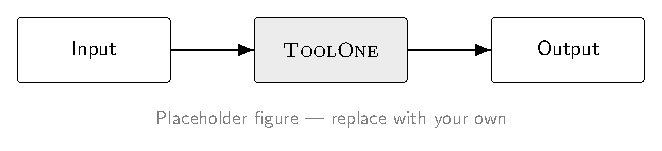
\includegraphics[width=0.75\linewidth]{figures/overview}
  \caption{Overview of \toolone.  Replace this placeholder with your
  own figure.}
  \label{fig:example-one-overview}
\end{figure}

Code listings can be typeset with the \latexpackage{listings}
package, configured in \file{main.tex}:

\begin{lstlisting}[caption={An example listing.},label=lst:example-one]
def solve(problem):
    context = select_context(problem)
    return generate_solution(problem, context)
\end{lstlisting}
